\section{Interaktion der Komponenten}
Auf Basis der Use Cases aus dem Analysedokument wird in diesem Kapitel die Interaktion der einzelnen Komponenten aus Kapitel 1 betrachtet. Dabei liegt der Fokus vor allem auf der Interaktion zwischen dem \emph{Server} und der \emph{RobotUnit}. Die Use Cases innerhalb der Komponenten werden in Kapitel 8 näher ausgeführt. \\


\subsection*{Interaktion bei Ausführung von \emph{Take Patient To Hospital & Select Best Match}}

Zuallerst fragt das \emph{Hospital} über Use Case 8: Check availability den \emph{Server} an, ob überhaupt ein \emph{Robot} verfügbar ist. Dann läuft die Auswahl eines \emph{Robots} nach Choose Robot wie im Diagramm beschrieben folgendermaßen ab: Bei einer neu eingehenden \emph{Destination} sendet der Server mit getSensorData(task) Anfragen an alle zur Verfügung stehenden \emph{Robots} (im Diagramm sind beispielhaft zwei angeführt, der Aufruf findet asynchron statt). Die \emph{Robots} führen dann Use Case 3: Read Sensors aus. Dabei sammeln sie alle notwendigen Informationen von ihren Hardwareschnittstellen, wie Ladestand und Nähe zum Ziel, die der \emph{Server} benötigt um den bestmöglichste \emph{Robot} auszuwählen. Sie warten auf das Zusammentragen der Daten, also das Abschließen des internen Loop-Prozesses, bis sie eine Nachricht mit den Informationen an den \emph{Server} zurücksenden; erst dann kann der \emph{Server} aufgrund der übermittelten Daten beurteilen, welcher \emph{Robot} am besten geeignet ist, den Patienten abzuholen und entsendet ihn zu den Zielkoordinaten (Use Case 7: Assign Task). Daraufhin folgt der Ablauf wieder vollständig dem Use Case Take Patient To Hospital. Wenn der \emph{Robot} nach Anfrageannahme und Fahrvorgang beim Patienten ankommt (arrived()) wird dabei immer auf die nächste direkte Bestätigung gewartet, damit das Warten nicht als eigene Sequenz verwenden muss. Dies setzt der Ausgangspunkt für den Use Case 9: Inform about boarding. Denn sobald der Patient sicher auf dem Roboter gebracht wurde, meldet das \emph{Hospital} dies unverzüglich über dem \emph{Server} an den \emph{Robot} zurück. Im Gegenzug existiert ebenso der Use Case 5: Inform about arrival, bei dem der \emph{Robot} sobald er das Krankenhaus erreicht hat, die Information über die Ankunft an den \emph{Server} weiterleitet, um die sofortige Versorgung des Patienten zu sichern.

\begin{figure}[H]
	\centering
	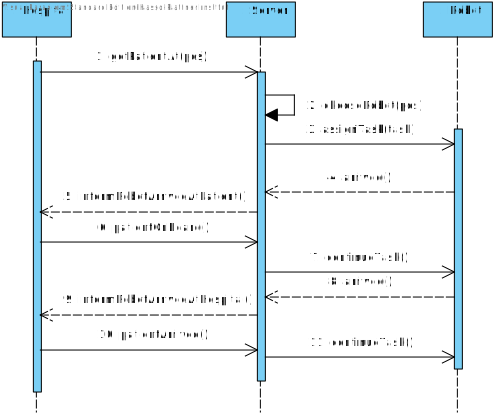
\includegraphics[width=0.9\textwidth]{img/1-Analyse-2-TakePatientToHospital}
	\caption{\emph{Take Patient To Hospital}-Sequenzdiagramm}
	\label{SequenzDiagrammInteraktion}
\end{figure}



\begin{figure}[H]
	\centering
	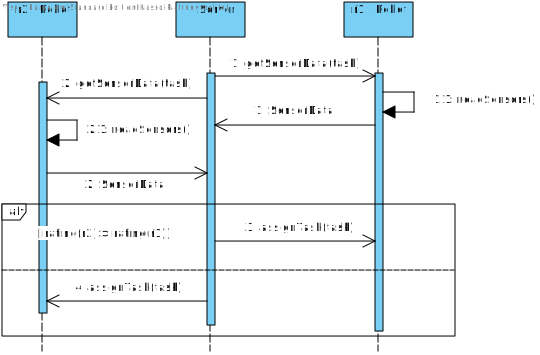
\includegraphics[width=0.9\textwidth]{img/0-Entwurf-2-ChooseRob}
	\caption{\emph{Select Best Match}-Sequenzdiagramm}
	\label{SequenzDiagrammInteraktion}
\end{figure}
